%        File: WeeklyResearchReport_4_19_21.tex
%     Created: Mon Apr 19 08:00 AM 2021 E
% Last Change: Mon Apr 19 08:00 AM 2021 E
%
\documentclass[a4paper]{article}
\usepackage{mathtools}
\usepackage{verbatim}
\usepackage{graphicx}
\usepackage{tabularx}
\usepackage{pgfplots}
\usepackage{adjustbox}
\usepackage{booktabs}
\makeatletter
\let\latex@xfloat=\@xfloat
\def\@xfloat #1[#2]{%
    \latex@xfloat #1[#2]%
    \def\baselinestretch{1}
    \@normalsize\normalsize
    \normalsize
}
\makeatother
\usepackage{amsmath}
\usepackage{mathtools}
\usepackage{epigraph}
\usepackage{cancel}
\usepackage{xcolor}
\newcommand\Ccancel[2][black]{\renewcommand\CancelColor{\color{#1}}\cancel{#2}}
\usepackage{algorithm}
\usepackage{graphicx}
\usepackage[noend]{algpseudocode}
\usepackage{gnuplot-lua-tikz}
\usepackage[utf8]{inputenc}
\usepackage{pgfplots}
\usepackage{tabularx}
\DeclareUnicodeCharacter{2212}{−}
\usepgfplotslibrary{groupplots,dateplot}
\usetikzlibrary{patterns,shapes.arrows}
\pgfplotsset{compat=newest}
\begin{document}
\begin{titlepage}

    \title{
    Daily Research Report}

    \author{ Jeffrey Severino \\
        University of Toledo \\
        Toledo, OH  43606 \\
    email: jseveri@rockets.utoledo.edu}


    \maketitle

\end{titlepage}
\section{Current Research Direction}
Automate the post processing for the axial wavenumbers such that the code 
verification is easier for the user.

\section{Research Performed}
% Scatter plots for axial wavenumbers                                           
\begin{figure}                                                                 
    \centering                                                                 
    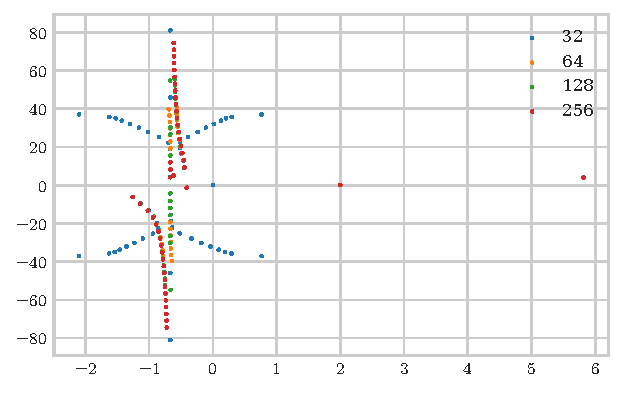
\includegraphics[width=\textwidth]{/home/jeff-severino/SWIRL/CodeRun/03-plotReport/tex-outputs/gam.nonconv.scatter32.pdf}
    \caption{Discrete Acoustic Disturbances: Cylinder, Uniform Mean Flow with Liner (2nd order scheme).}
\end{figure}                                                                   




% Scatter plots for axial wavenumbers                                           
\begin{figure}                                                                 
    \centering                                                                 
    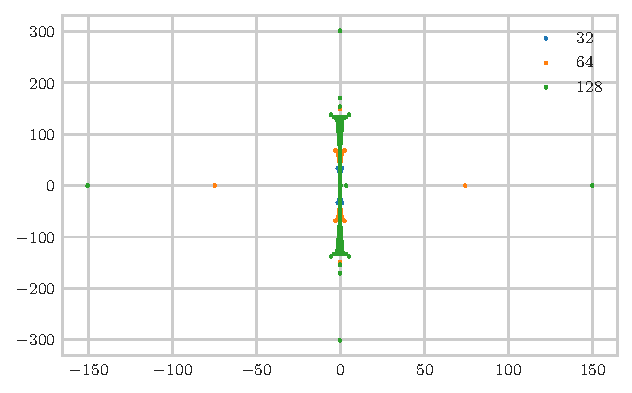
\includegraphics[width=\textwidth]{/home/jeff-severino/SWIRL/CodeRun/03-plotReport/tex-outputs/gam.nonconv.scatter_4th_order_comp.pdf}
    \caption{Discrete Acoustic Disturbances: Cylinder, Uniform Mean Flow with Liner (4th order scheme).}
\end{figure}                                                                   

\begin{figure}
    \centering
    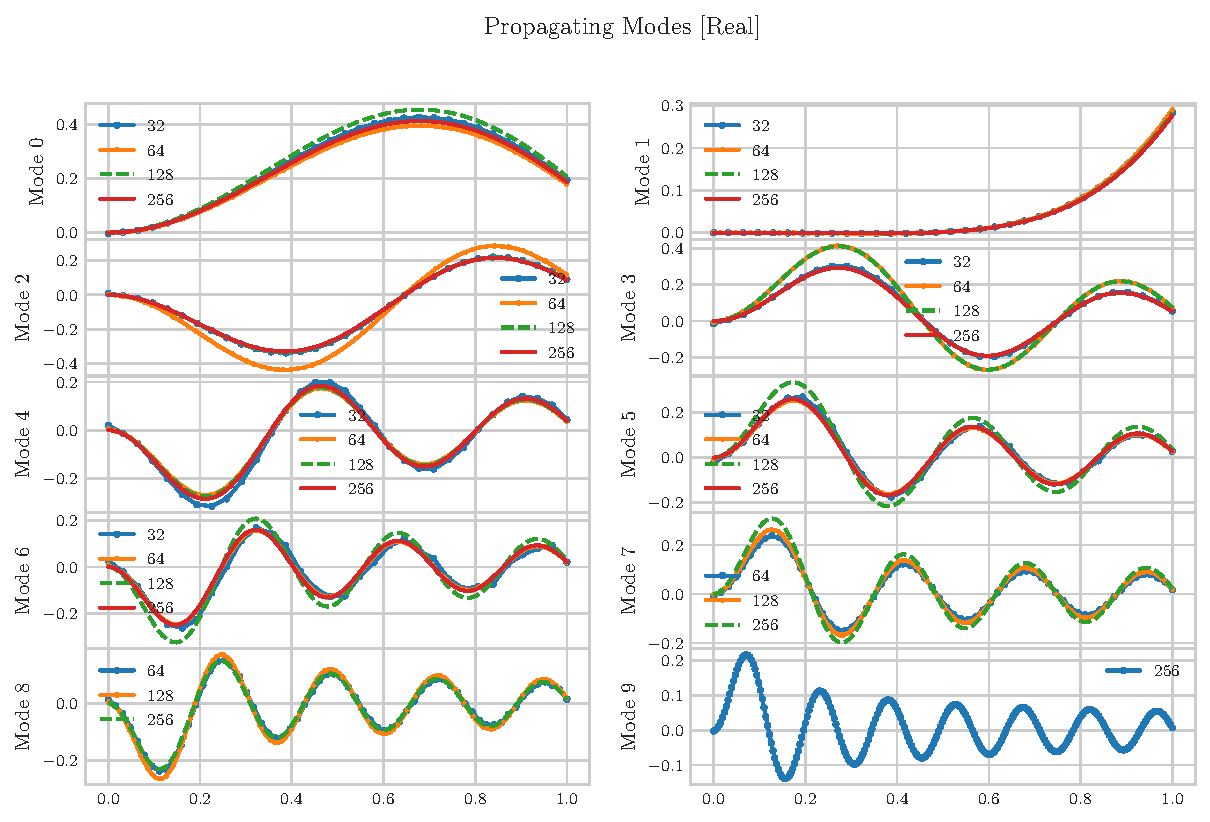
\includegraphics[width=\textwidth]{/home/jeff-severino/SWIRL/CodeRun/03-plotReport/tex-outputs/egv_prop_re.pdf}
\end{figure}

The scatter plots show the difference between the second order and fourth
order schemes. Note how the cut on line is much more defined. The plots of the propagating 
and decaying modes are shown below. For Mode 1, there is a zero crossing early that
is hard to see but is apparent in the tables of data that there is indeed a sign

 \begin{figure}
     \centering
     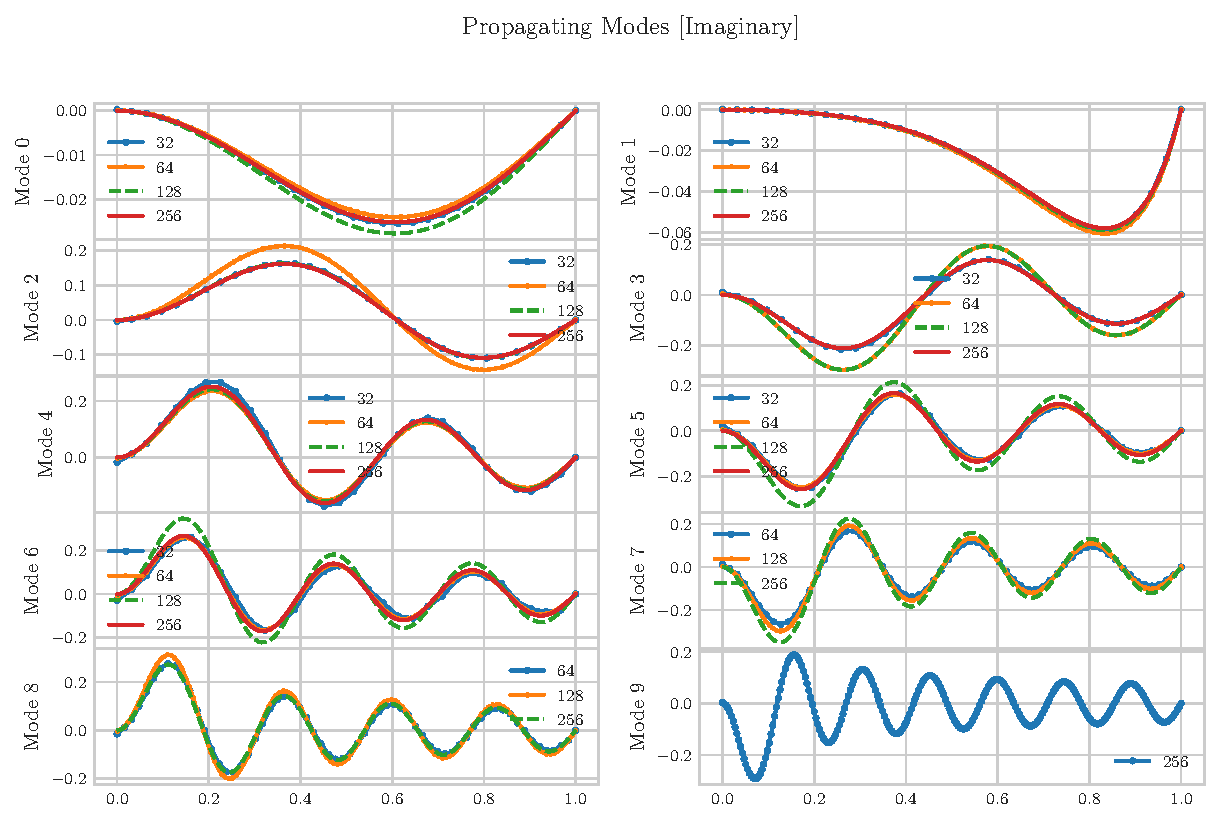
\includegraphics[width=\textwidth]{/home/jeff-severino/SWIRL/CodeRun/03-plotReport/tex-outputs/egv_prop_im.pdf}
 \end{figure}


 \begin{figure}
     \centering
     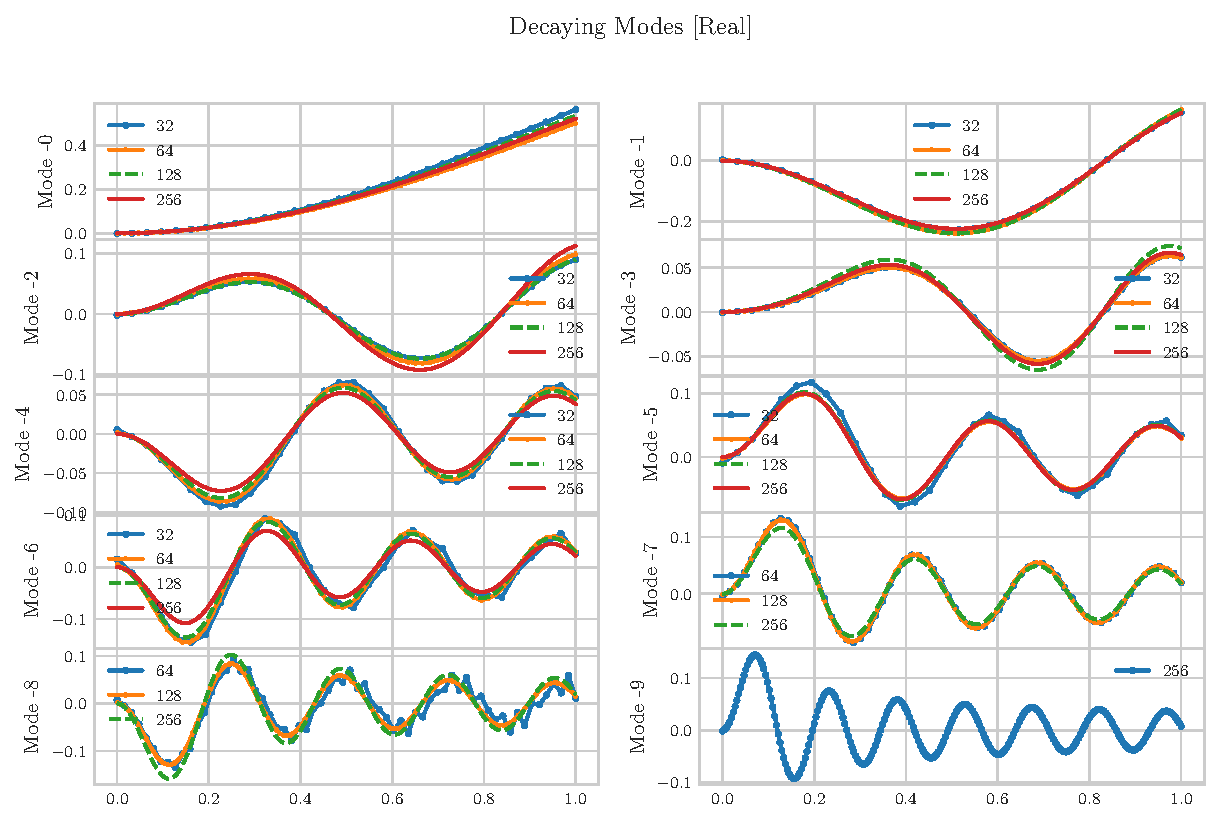
\includegraphics[width=\textwidth]{/home/jeff-severino/SWIRL/CodeRun/03-plotReport/tex-outputs/egv_decay_re.pdf}
 \end{figure}


 \begin{figure}
     \centering
     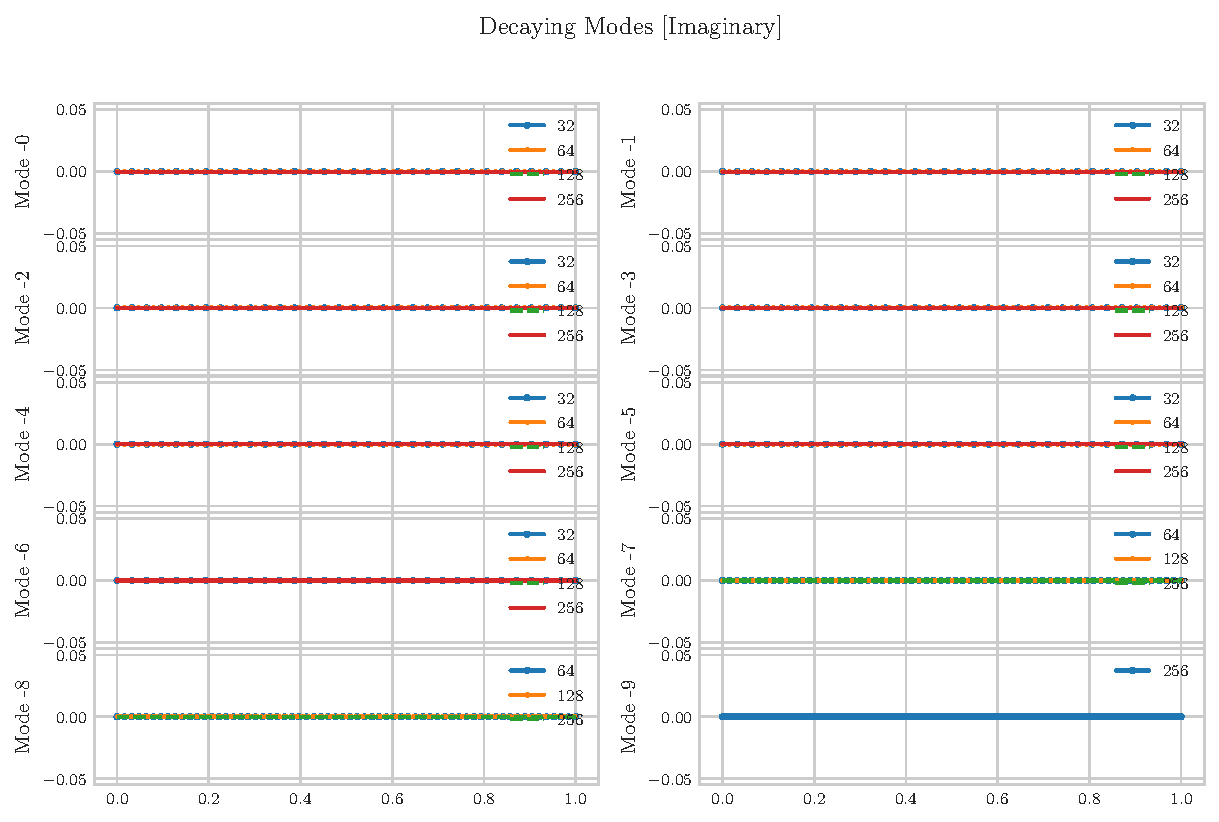
\includegraphics[width=\textwidth]{/home/jeff-severino/SWIRL/CodeRun/03-plotReport/tex-outputs/egv_decay_im.pdf}
 \end{figure}



\section{Planned Research}
A for loop and naming convention is needed to loop through all the possible data 
sets so there isnt error from the user.
\end{document}


